\documentclass[dvipsnames,border=3pt]{standalone}
\usepackage{tikz}
\usetikzlibrary{arrows}
\usetikzlibrary{shapes}
\usepackage{enumitem}
\usepackage{bm}
\usepackage{mathdots}
\usepackage{amsmath}
\usetikzlibrary{shadings}
\usetikzlibrary{decorations.pathreplacing}
\usepackage{helvet}
\usetikzlibrary{arrows.meta}
\usepackage{graphicx}
\usepackage{pgfplots}
\usepackage{pgfplotstable}
\usepackage{filecontents}
\usetikzlibrary{plotmarks}
\pgfplotsset{compat=newest}

\renewcommand{\familydefault}{\sfdefault}

\definecolor{mylightgray}{cmyk}{0,0,0,0.1}
\definecolor{mygreen}{rgb}{0,109,44}
\usetikzlibrary{arrows,decorations.pathmorphing,backgrounds,fit,positioning,shapes.symbols,chains}

\begin{document}

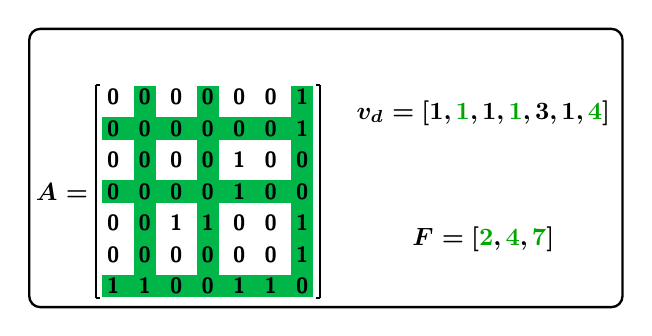
\begin{tikzpicture}
    % trim=left botm right top
    
    %%%%%%%%%%%%%%%%%%%%%%%%%%%%%%%%%%%%%%%%%%%%%%%%%%%%%%%%%%%%%%%%%%%%%%%%%%%%%%%%%%%%%%%%%%%%%%%%%%
    %%%%%%%%%%%%%%%%%%%%%%%%%%%%%%%%%%%%%%%%%%% box 2 %%%%%%%%%%%%%%%%%%%%%%%%%%%%%%%%%%%%%%%%%%%%%%%%
    %%%%%%%%%%%%%%%%%%%%%%%%%%%%%%%%%%%%%%%%%%%%%%%%%%%%%%%%%%%%%%%%%%%%%%%%%%%%%%%%%%%%%%%%%%%%%%%%%%
    
    \node[draw, rounded corners=4, line width=0.3mm, text width=7.3cm, text height=3.3cm] at (0.2,-4.7) {};
    %\node[circle,draw,line width=0.2mm,xscale=1.2,yscale=1.2,fill=GreenYellow] at (-3.3,-3.595) {};
    %\node at (-3.3,-3.595) {\textbf{2}};
    
    %%%%%%%%%%%%%%%%%%%%%%%%%%%%%%%%%%%%%%%%%%%%%%%%%%%%%%%%%%%%%%%%%%%%%%%%%%%%%%%%%%%%%%%%%%%%%%%%%%
    %%%%%%%%%%%%%%%%%%%%%%%%%%%%%%%%%%%%%%%%%%% box 2 %%%%%%%%%%%%%%%%%%%%%%%%%%%%%%%%%%%%%%%%%%%%%%%%
    %%%%%%%%%%%%%%%%%%%%%%%%%%%%%%%%%%%%%%%%%%%%%%%%%%%%%%%%%%%%%%%%%%%%%%%%%%%%%%%%%%%%%%%%%%%%%%%%%%
    
    %%%%%%%%%%%%%%%%%%%%%%%%%%%%%%%%%%%%%%%%%%%%%%%%%%%%%%%%%%%%%%%%%%%%%%%%%%%%%%%%%%%%%%%%%%%%%%%%%%
    %%%%%%%%%%%%%%%%%%%%%%%%%%%%%%%%%%%%% adjacency matrix %%%%%%%%%%%%%%%%%%%%%%%%%%%%%%%%%%%%%%%%%%%
    %%%%%%%%%%%%%%%%%%%%%%%%%%%%%%%%%%%%%%%%%%%%%%%%%%%%%%%%%%%%%%%%%%%%%%%%%%%%%%%%%%%%%%%%%%%%%%%%%%
    
    %\node[draw, rounded corners=2, line width=0.2mm,text height=0.2cm,text width=1.95cm,fill=gray!50,shading angle=45] at (-1.38,-3.6) {};
    %\node[xscale=0.7,yscale=0.7] at (-1.38,-3.6) {\textbf{Adjacency Matrix}};
    
    %%%%%%%%%%%%%%%%%%%%%%%%%%%%%%%%%%%%%%%%%%%%%%%%%%%%%%%%% matrix left
    
    % row and col 2 highlighting
    \node[fill={rgb:red,0;green,109;blue,44},text height=2.45cm,text width=0.05cm] at (-2.1,-5) {}; % col 2
    \node[fill={rgb:red,0;green,109;blue,44},text height=0.05cm,text width=2.45cm] at (-1.3,-4.2) {}; % row 2
    
    % row and col 5 highlighting
    \node[fill={rgb:red,0;green,109;blue,44},text height=2.45cm,text width=0.05cm] at (-1.3,-5) {}; % col 5
    \node[fill={rgb:red,0;green,109;blue,44},text height=0.05cm,text width=2.45cm] at (-1.3,-5) {}; % row 5
    
    % row and col 7 highlighting
    \node[fill={rgb:red,0;green,109;blue,44},text height=2.45cm,text width=0.05cm] at (-0.1,-5) {}; % col 7
    \node[fill={rgb:red,0;green,109;blue,44},text height=0.05cm,text width=2.45cm] at (-1.3,-6.2) {}; % row 7
    
    % row 1
    \node[xscale=0.8,yscale=0.8] at (-2.5,-3.8) {\textbf{0}};
    \node[xscale=0.8,yscale=0.8] at (-2.1,-3.8) {\textbf{0}};
    \node[xscale=0.8,yscale=0.8] at (-1.7,-3.8) {\textbf{0}};
    \node[xscale=0.8,yscale=0.8] at (-1.3,-3.8) {\textbf{0}};
    \node[xscale=0.8,yscale=0.8] at (-0.9,-3.8) {\textbf{0}};
    \node[xscale=0.8,yscale=0.8] at (-0.5,-3.8) {\textbf{0}};
    \node[xscale=0.8,yscale=0.8] at (-0.1,-3.8) {\textbf{1}};
    
    % row 2
    \node[xscale=0.8,yscale=0.8] at (-2.5,-4.2) {\textbf{0}};
    \node[xscale=0.8,yscale=0.8] at (-2.1,-4.2) {\textbf{0}};
    \node[xscale=0.8,yscale=0.8] at (-1.7,-4.2) {\textbf{0}};
    \node[xscale=0.8,yscale=0.8] at (-1.3,-4.2) {\textbf{0}};
    \node[xscale=0.8,yscale=0.8] at (-0.9,-4.2) {\textbf{0}};
    \node[xscale=0.8,yscale=0.8] at (-0.5,-4.2) {\textbf{0}};
    \node[xscale=0.8,yscale=0.8] at (-0.1,-4.2) {\textbf{1}};
    
    % row 3
    \node[xscale=0.8,yscale=0.8] at (-2.5,-4.6) {\textbf{0}};
    \node[xscale=0.8,yscale=0.8] at (-2.1,-4.6) {\textbf{0}};
    \node[xscale=0.8,yscale=0.8] at (-1.7,-4.6) {\textbf{0}};
    \node[xscale=0.8,yscale=0.8] at (-1.3,-4.6) {\textbf{0}};
    \node[xscale=0.8,yscale=0.8] at (-0.9,-4.6) {\textbf{1}};
    \node[xscale=0.8,yscale=0.8] at (-0.5,-4.6) {\textbf{0}};
    \node[xscale=0.8,yscale=0.8] at (-0.1,-4.6) {\textbf{0}};
    
    % row 4
    \node[xscale=0.8,yscale=0.8] at (-2.5,-5) {\textbf{0}};
    \node[xscale=0.8,yscale=0.8] at (-2.1,-5) {\textbf{0}};
    \node[xscale=0.8,yscale=0.8] at (-1.7,-5) {\textbf{0}};
    \node[xscale=0.8,yscale=0.8] at (-1.3,-5) {\textbf{0}};
    \node[xscale=0.8,yscale=0.8] at (-0.9,-5) {\textbf{1}};
    \node[xscale=0.8,yscale=0.8] at (-0.5,-5) {\textbf{0}};
    \node[xscale=0.8,yscale=0.8] at (-0.1,-5) {\textbf{0}};
    
    % row 5
    \node[xscale=0.8,yscale=0.8] at (-2.5,-5.4) {\textbf{0}};
    \node[xscale=0.8,yscale=0.8] at (-2.1,-5.4) {\textbf{0}};
    \node[xscale=0.8,yscale=0.8] at (-1.7,-5.4) {\textbf{1}};
    \node[xscale=0.8,yscale=0.8] at (-1.3,-5.4) {\textbf{1}};
    \node[xscale=0.8,yscale=0.8] at (-0.9,-5.4) {\textbf{0}};
    \node[xscale=0.8,yscale=0.8] at (-0.5,-5.4) {\textbf{0}};
    \node[xscale=0.8,yscale=0.8] at (-0.1,-5.4) {\textbf{1}};
    
    % row 6
    \node[xscale=0.8,yscale=0.8] at (-2.5,-5.8) {\textbf{0}};
    \node[xscale=0.8,yscale=0.8] at (-2.1,-5.8) {\textbf{0}};
    \node[xscale=0.8,yscale=0.8] at (-1.7,-5.8) {\textbf{0}};
    \node[xscale=0.8,yscale=0.8] at (-1.3,-5.8) {\textbf{0}};
    \node[xscale=0.8,yscale=0.8] at (-0.9,-5.8) {\textbf{0}};
    \node[xscale=0.8,yscale=0.8] at (-0.5,-5.8) {\textbf{0}};
    \node[xscale=0.8,yscale=0.8] at (-0.1,-5.8) {\textbf{1}};
    
    % row 7
    \node[xscale=0.8,yscale=0.8] at (-2.5,-6.2) {\textbf{1}};
    \node[xscale=0.8,yscale=0.8] at (-2.1,-6.2) {\textbf{1}};
    \node[xscale=0.8,yscale=0.8] at (-1.7,-6.2) {\textbf{0}};
    \node[xscale=0.8,yscale=0.8] at (-1.3,-6.2) {\textbf{0}};
    \node[xscale=0.8,yscale=0.8] at (-0.9,-6.2) {\textbf{1}};
    \node[xscale=0.8,yscale=0.8] at (-0.5,-6.2) {\textbf{1}};
    \node[xscale=0.8,yscale=0.8] at (-0.1,-6.2) {\textbf{0}};
    
    \draw[line width=0.25mm] (-2.72,-3.65) -- (-2.72,-6.35);
    \draw[line width=0.25mm] (-2.72,-3.65) -- (-2.67,-3.65);
    \draw[line width=0.25mm] (-2.72,-6.35) -- (-2.67,-6.35);
    
    \draw[line width=0.25mm] (0.12,-3.65) -- (0.12,-6.35);
    \draw[line width=0.25mm] (0.12,-3.65) -- (0.07,-3.65);
    \draw[line width=0.25mm] (0.12,-6.35) -- (0.07,-6.35);
    
    \node[xscale=0.9,yscale=0.9] at (-3.15,-5.0) {\bm{$A$} \bm{$=$}};
    %%%%%%%%%%%%%%%%%%%%%%%%%%%%%%%%%%%%%%%%%%%%%%%%%%%%%%%%% matrix left
    
    %%%%%%%%%%%%%%%%%%%%%%%%%%%%%%%%%%%%%%%%%%%%%%%%%%%%%%%%% matrix right
    
    % row 1
    %\node[xscale=0.5,yscale=0.5] at (1.36,-4.5) {\textbf{0}};
    %\node[xscale=0.5,yscale=0.5] at (1.56,-4.5) {\textbf{1}};
    %\node[xscale=0.5,yscale=0.5] at (1.76,-4.5) {\textbf{0}};
    %\node[xscale=0.5,yscale=0.5] at (1.96,-4.5) {\textbf{0}};
    %\node[xscale=0.5,yscale=0.5] at (2.16,-4.5) {\textbf{0}};
    %\node[xscale=0.5,yscale=0.5] at (2.36,-4.5) {\textbf{0}};
    %\node[xscale=0.5,yscale=0.5] at (2.56,-4.5) {\textbf{1}};
    
    % row 2
    %\node[xscale=0.5,yscale=0.5] at (1.36,-4.7) {\textbf{1}};
    %\node[xscale=0.5,yscale=0.5] at (1.56,-4.7) {\textbf{0}};
    %\node[xscale=0.5,yscale=0.5] at (1.76,-4.7) {\textbf{1}};
    %\node[xscale=0.5,yscale=0.5] at (1.96,-4.7) {\textbf{0}};
    %\node[xscale=0.5,yscale=0.5] at (2.16,-4.7) {\textbf{0}};
    %\node[xscale=0.5,yscale=0.5] at (2.36,-4.7) {\textbf{0}};
    %\node[xscale=0.5,yscale=0.5] at (2.56,-4.7) {\textbf{0}};
    
    % row 3
    %\node[xscale=0.5,yscale=0.5] at (1.36,-4.9) {\textbf{0}};
    %\node[xscale=0.5,yscale=0.5] at (1.56,-4.9) {\textbf{1}};
    %\node[xscale=0.5,yscale=0.5] at (1.76,-4.9) {\textbf{0}};
    %\node[xscale=0.5,yscale=0.5] at (1.96,-4.9) {\textbf{1}};
    %\node[xscale=0.5,yscale=0.5] at (2.16,-4.9) {\textbf{0}};
    %\node[xscale=0.5,yscale=0.5] at (2.36,-4.9) {\textbf{0}};
    %\node[xscale=0.5,yscale=0.5] at (2.56,-4.9) {\textbf{1}};
    
    % row 4
    %\node[xscale=0.5,yscale=0.5] at (1.36,-5.1) {\textbf{0}};
    %\node[xscale=0.5,yscale=0.5] at (1.56,-5.1) {\textbf{0}};
    %\node[xscale=0.5,yscale=0.5] at (1.76,-5.1) {\textbf{1}};
    %\node[xscale=0.5,yscale=0.5] at (1.96,-5.1) {\textbf{0}};
    %\node[xscale=0.5,yscale=0.5] at (2.16,-5.1) {\textbf{0}};
    %\node[xscale=0.5,yscale=0.5] at (2.36,-5.1) {\textbf{0}};
    %\node[xscale=0.5,yscale=0.5] at (2.56,-5.1) {\textbf{0}};
    
    % row 5
    %\node[xscale=0.5,yscale=0.5] at (1.36,-5.3) {\textbf{0}};
    %\node[xscale=0.5,yscale=0.5] at (1.56,-5.3) {\textbf{0}};
    %\node[xscale=0.5,yscale=0.5] at (1.76,-5.3) {\textbf{0}};
    %\node[xscale=0.5,yscale=0.5] at (1.96,-5.3) {\textbf{0}};
    %\node[xscale=0.5,yscale=0.5] at (2.16,-5.3) {\textbf{0}};
    %\node[xscale=0.5,yscale=0.5] at (2.36,-5.3) {\textbf{0}};
    %\node[xscale=0.5,yscale=0.5] at (2.56,-5.3) {\textbf{0}};
    
    % row 6
    %\node[xscale=0.5,yscale=0.5] at (1.36,-5.5) {\textbf{0}};
    %\node[xscale=0.5,yscale=0.5] at (1.56,-5.5) {\textbf{0}};
    %\node[xscale=0.5,yscale=0.5] at (1.76,-5.5) {\textbf{0}};
    %\node[xscale=0.5,yscale=0.5] at (1.96,-5.5) {\textbf{0}};
    %\node[xscale=0.5,yscale=0.5] at (2.16,-5.5) {\textbf{0}};
    %\node[xscale=0.5,yscale=0.5] at (2.36,-5.5) {\textbf{0}};
    %\node[xscale=0.5,yscale=0.5] at (2.56,-5.5) {\textbf{1}};
    
    % row 7
    %\node[xscale=0.5,yscale=0.5] at (1.36,-5.7) {\textbf{1}};
    %\node[xscale=0.5,yscale=0.5] at (1.56,-5.7) {\textbf{0}};
    %\node[xscale=0.5,yscale=0.5] at (1.76,-5.7) {\textbf{1}};
    %\node[xscale=0.5,yscale=0.5] at (1.96,-5.7) {\textbf{0}};
    %\node[xscale=0.5,yscale=0.5] at (2.16,-5.7) {\textbf{0}};
    %\node[xscale=0.5,yscale=0.5] at (2.36,-5.7) {\textbf{1}};
    %\node[xscale=0.5,yscale=0.5] at (2.56,-5.7) {\textbf{0}};
    
    %\draw[line width=0.2mm] (1.24,-4.4) -- (1.24,-5.8);
    %\draw[line width=0.2mm] (1.24,-4.4) -- (1.29,-4.4);
    %\draw[line width=0.2mm] (1.24,-5.8) -- (1.29,-5.8);
    
    %\draw[line width=0.2mm] (2.68,-4.4) -- (2.68,-5.8);
    %\draw[line width=0.2mm] (2.68,-4.4) -- (2.63,-4.4);
    %\draw[line width=0.2mm] (2.68,-5.8) -- (2.63,-5.8);
    
    %\node[xscale=0.7,yscale=0.7] at (0.88,-5.1) {\textcolor{cyan}{\bm{$A$}} \bm{$=$}};
    
    %%%%%%%%%%%%%%%%%%%%%%%%%%%%%%%%%%%%%%%%%%%%%%%%%%%%%%%%% matrix right
    
    %%%%%%%%%%%%%%%%%%%%%%%%%%%%%%%%%%%%%%%%%%%%%%%%%%%%%%%%%%%%%%%%%%%%%%%%%%%%%%%%%%%%%%%%%%%%%%%%%%
    %%%%%%%%%%%%%%%%%%%%%%%%%%%%%%%%%%%%% adjacency matrix %%%%%%%%%%%%%%%%%%%%%%%%%%%%%%%%%%%%%%%%%%%
    %%%%%%%%%%%%%%%%%%%%%%%%%%%%%%%%%%%%%%%%%%%%%%%%%%%%%%%%%%%%%%%%%%%%%%%%%%%%%%%%%%%%%%%%%%%%%%%%%%
    
    %%%%%%%%%%%%%%%%%%%%%%%%%%%%%%%%%%%%%%%%%%%%%%%%%%%%%%%%%%%%%%%%%%%%%%%%%%%%%%%%%%%%%%%%%%%%%%%%%%
    %%%%%%%%%%%%%%%%%%%%%%%%%%%%%%%%%%%%%%%% degree vector %%%%%%%%%%%%%%%%%%%%%%%%%%%%%%%%%%%%%%%%%%%
    %%%%%%%%%%%%%%%%%%%%%%%%%%%%%%%%%%%%%%%%%%%%%%%%%%%%%%%%%%%%%%%%%%%%%%%%%%%%%%%%%%%%%%%%%%%%%%%%%%
    
    %\node[draw, rounded corners=2, line width=0.2mm,text height=0.2cm,text width=1.72cm,fill=gray!50,shading angle=45] at (1.9,-3.6) {};
    %\node[xscale=0.7,yscale=0.7] at (1.9,-3.6) {\textbf{Degree Vector}};
    
    \node[xscale=0.9,yscale=0.9] at (2.2,-4) {\bm{$v_d$} \bm{$ = [1, \textcolor{black!35!green}{1}, 1, \textcolor{black!35!green}{1}, 3, 1, \textcolor{black!35!green}{4}]$}};
    
    %\node[xscale=0.7,yscale=0.7] at (2,-8) {\textcolor{cyan}{\bm{$v_d$}} \bm{$ = [2, 2, 3, 1, 0, 1, 3]^\textbf{T}$}};
    
    %%%%%%%%%%%%%%%%%%%%%%%%%%%%%%%%%%%%%%%%%%%%%%%%%%%%%%%%%%%%%%%%%%%%%%%%%%%%%%%%%%%%%%%%%%%%%%%%%%
    %%%%%%%%%%%%%%%%%%%%%%%%%%%%%%%%%%%%%%%% degree vector %%%%%%%%%%%%%%%%%%%%%%%%%%%%%%%%%%%%%%%%%%%
    %%%%%%%%%%%%%%%%%%%%%%%%%%%%%%%%%%%%%%%%%%%%%%%%%%%%%%%%%%%%%%%%%%%%%%%%%%%%%%%%%%%%%%%%%%%%%%%%%%
    
    %%%%%%%%%%%%%%%%%%%%%%%%%%%%%%%%%%%%%%%%%%%%%%%%%%%%%%%%%%%%%%%%%%%%%%%%%%%%%%%%%%%%%%%%%%%%%%%%%%
    %%%%%%%%%%%%%%%%%%%%%%%%%%%%%%%%%%%%% functional features %%%%%%%%%%%%%%%%%%%%%%%%%%%%%%%%%%%%%%%%
    %%%%%%%%%%%%%%%%%%%%%%%%%%%%%%%%%%%%%%%%%%%%%%%%%%%%%%%%%%%%%%%%%%%%%%%%%%%%%%%%%%%%%%%%%%%%%%%%%%
    
    %\node[draw, rounded corners=2, line width=0.2mm,text height=0.2cm,text width=2.26cm,fill=gray!50,shading angle=45] at (1.9,-5.2) {};
    %\node[xscale=0.7,yscale=0.7] at (1.9,-5.2) {\textbf{Functional Features}};
    
    \node[xscale=0.9,yscale=0.9] at (2.2,-5.6) {\bm{$F$} \bm{$ = [\textcolor{black!35!green}{2}, \textcolor{black!35!green}{4}, \textcolor{black!35!green}{7}]$}};
    
    %\node[xscale=0.7,yscale=0.7] at (2,-10.2) {\textcolor{cyan}{\bm{$f$}} \bm{$ = [1, 3, 6]^\textbf{T}$}};
    
    %%%%%%%%%%%%%%%%%%%%%%%%%%%%%%%%%%%%%%%%%%%%%%%%%%%%%%%%%%%%%%%%%%%%%%%%%%%%%%%%%%%%%%%%%%%%%%%%%%
    %%%%%%%%%%%%%%%%%%%%%%%%%%%%%%%%%%%%% functional features %%%%%%%%%%%%%%%%%%%%%%%%%%%%%%%%%%%%%%%%
    %%%%%%%%%%%%%%%%%%%%%%%%%%%%%%%%%%%%%%%%%%%%%%%%%%%%%%%%%%%%%%%%%%%%%%%%%%%%%%%%%%%%%%%%%%%%%%%%%%
    
    \end{tikzpicture}
    
\end{document}